% This must be in the first 5 lines to tell arXiv to use pdfLaTeX, which is strongly recommended.
\pdfoutput=1

\documentclass[11pt]{article}

% Change "review" to "final" to generate the final (sometimes called camera-ready) version.
% Change to "preprint" to generate a non-anonymous version with page numbers.
%\usepackage[review]{acl}
\usepackage{acl}
\usepackage{graphicx}
\usepackage{times}
\usepackage{latexsym}
\usepackage{booktabs}
\usepackage[T1]{fontenc}
\usepackage[utf8]{inputenc}
\usepackage{microtype}
\usepackage{inconsolata}

\title{A Text Has No Taste: Synesthetic Probing of Language Models\\ and the Absent Referent}

\author{Omar Cherif \\
  LORIA \\
  \texttt{mohamed.cherif@inria.fr} \\\And
  Christophe Cerisara \\
  LORIA\\
  \texttt{christophe.cerisara@loria.fr}  \\\AND
  Julien Falgas \\
  CREM, Université de Lorraine \\
  \texttt{julien.falgas@univ-lorraine.fr} \\}

\begin{document}
\maketitle

\begin{abstract}
We ask a language model whether a text is \emph{purple}, \emph{salty}, \emph{grainy}, \emph{nasal} or \emph{smoky}, and read the difference between the logits of ``yes'' and ``no'' as a feature. With only twenty such \emph{synesthetic} questions spanning the five senses, a linear classifier reaches $0.93$ accuracy on sentiment (IMDB) and beats a random-word control by large margins on four datasets. Crucially, we manipulate the \emph{metaphoricity} of the questions: predicates such as \emph{purple} or \emph{umami} carry no conventional figurative meaning, unlike \emph{dark} or \emph{bitter}. While more metaphorical predicates are individually somewhat more useful, low-metaphoricity sensory probes---which can only be answered by reference to a perception the model never had---remain strongly informative on every task. We read this through Saussure: a text-only model has no \emph{referent}, so sensory predicates are unconstrained signifiers whose value comes from differences within the language system, not from the senses. A red text and an acidic text are, for the model, equally sayable.
\end{abstract}

\section{Introduction}
A language model can be asked whether a text is ``acidic'', ``rough'' or ``purple''. There is no fact of the matter: a string of characters has no taste, no texture and no colour. Yet the model never refuses to answer, and---as we show---its graded answers carry reliable information about the text. This paper takes that small observation seriously.

We extend the feature-generation approach of \citet{florescuAlgorithmicallyGeneratingNew2019}, in which an LLM is queried with simple questions about a text and the answer logits are used as features for a downstream classifier. Out of the many question types one could ask, we isolate the most theoretically puzzling one: \emph{synesthetic} questions, which describe a text through a sensory modality \citep{cytowicSynesthesiaUnionSenses2002}. Because the model perceives only text, such questions cannot be grounded in perception; they should be meaningless. They are not.

Our contributions are: (i) a controlled set of $20$ synesthetic questions (four per sense) selected for \emph{low metaphoricity}, i.e.\ minimal conventional figurative meaning, together with a matched high-metaphoricity set; (ii) an evaluation on four datasets spanning sentiment, topic and emotion, showing that synesthetic features classify far above a random-word control and chance, and rival TF--IDF on affective tasks; (iii) an analysis showing that usefulness only weakly depends on metaphoricity---non-figurative sensory probes still work---and (iv) a reading of these results through Saussure's notion of the sign without a referent.

\section{Background and related work}
\paragraph{Synesthesia in perception and in language.}
Synesthesia is a phenomenon in which a stimulus in one sensory modality triggers a perception in another \citep{cytowicSynesthesiaUnionSenses2002}. Language is itself full of \emph{lexicalized} synesthetic transfers---a \emph{sweet} voice, a \emph{warm} colour---which follow regular cross-modal directionalities \citep{ullmann1957principles,striklievers2015synaesthesia,winter2019sensory}. These conventional metaphors are precisely what we want to control for: a feature that works because ``bitter'' already means ``resentful'' tells us about lexicalized semantics, not about synesthetic projection.

\paragraph{Meaning, form and grounding.}
Whether a system trained only on form can acquire meaning is contested \citep{benderkoller2020climbing,bender2021stochastic,bisk2020experience}, and connects to the older symbol grounding problem \citep{harnad1990symbol}. Our probe offers an empirical angle: sensory predicates are the clearest case of words whose meaning seems to require perceptual grounding, so they are an ideal stress test for ``form without referent''.

\paragraph{The Saussurean sign.}
For \citet{saussure1916cours}, the linguistic sign unites a signifier and a signified through an arbitrary relation, and the \emph{value} of a sign arises from its differences with other signs in the system (\emph{la langue}), not from any link to an external thing---the referent is bracketed. A distributional model in the sense of \citet{firth1957synopsis} is, in this light, a system of pure differential values. We argue this is exactly the regime in which our synesthetic questions operate.

\section{Method}
\subsection{Synesthetic questions and metaphoricity}
We write $20$ yes/no questions, four for each of the five senses (sight, taste, touch, hearing, smell). The questions are chosen to have \emph{low metaphoricity}: the predicate has little or no conventional non-physical meaning in English (e.g.\ \emph{purple}, \emph{umami}, \emph{starchy}, \emph{grainy}, \emph{nasal}, \emph{metallic}). We deliberately avoid predicates that are dead metaphors (\emph{dark}, \emph{bitter}, \emph{warm}, \emph{loud}, \emph{fishy}), and place those instead in a matched \emph{high-metaphoricity} set of $20$ questions. A third set of $10$ \emph{gibberish} probes (``does this text evoke the words: lantern, gravel, \dots'') acts as a control for whether \emph{any} probe carries information. All questions are listed in Appendix~\ref{sec:appendix}.

To measure metaphoricity independently of our own judgments, we also ask the model itself, for each predicate, whether it ``is often used figuratively or metaphorically to describe something non-physical'', and record the yes/no logit difference. This model-based score cleanly separates the two sets (high-metaphoricity predicates: \emph{warm} $+11.7$, \emph{dark} $+11.4$, \emph{sweet} $+10.9$; low: \emph{starchy} $-7.3$, \emph{minty} $-6.2$, \emph{nasal} $-6.0$), and is used in the analysis of Section~\ref{sec:meta}.

\subsection{Feature extraction}
Following \citet{florescuAlgorithmicallyGeneratingNew2019}, we present the text followed by a question and ask for a yes/no answer. Instead of decoding, we read the model's next-token logits at the answer position and define the feature as
\[
f_q(t) = \log\!\!\sum_{v\in\mathrm{YES}}\!\! e^{z_v} \;-\; \log\!\!\sum_{v\in\mathrm{NO}}\!\! e^{z_v},
\]
where $z$ are the logits and $\mathrm{YES}$/$\mathrm{NO}$ are the case and whitespace variants of ``yes''/``no''. Each text is thus mapped to a $20$-dimensional synesthetic feature vector. We use \texttt{google/gemma-4-E4B-it} \citep{gemma4_2026}, a recent instruction-tuned model, with greedy single-pass forward computations (no sampling).

\subsection{Datasets and classifier}
We use balanced subsets of $500$ examples (stratified by class) from four datasets covering distinct tasks: \textbf{IMDB} (sentiment, 2 classes), \textbf{AG~News} (topic, 4), \textbf{BBC~News} (topic, 5) and \textbf{Emotion} (affect, 6). Texts are truncated to $300$ words. On the resulting features we train a logistic regression with standardized inputs and report $5$-fold stratified cross-validation accuracy; we deliberately use a weak linear classifier so that performance reflects the information in the features rather than classifier capacity, and we verify that a small MLP gives equivalent results (Table~\ref{tab:zeroshot}). Baselines are the gibberish features, a TF--IDF (1--2-gram) logistic regression on the raw text, direct zero-shot classification, and the majority-class chance level.

\section{Results}
\paragraph{Synesthetic features classify, gibberish does not.}
Table~\ref{tab:main} and Figure~\ref{fig:groups} show that the $20$ low-polysemy synesthetic features are strongly predictive on every dataset, far above both chance and the random-word control. On IMDB they reach $0.88$ (vs.\ $0.66$ for gibberish and $0.79$ for TF--IDF); the full $40$-question set reaches $0.92$. On topic tasks TF--IDF wins (it is, after all, a lexical task), but synesthetic features still recover most of the signal from senses that have nothing to do with topics.

\begin{table}[t]
\centering\small
\begin{tabular}{lccccc}
\toprule
 & chance & \textsc{low} & \textsc{high} & \textsc{all} & \textsc{gib} \\
\midrule
IMDB     & .500 & .880 & \textbf{.934} & .924 & .660 \\
AG News  & .250 & .658 & .662 & \textbf{.710} & .558 \\
BBC      & .200 & .714 & .654 & \textbf{.768} & .504 \\
Emotion  & .167 & .287 & .390 & \textbf{.424} & .235 \\
\bottomrule
\end{tabular}
\caption{5-fold CV accuracy. \textsc{low}/\textsc{high}: 20 low-/high-metaphoricity synesthetic questions; \textsc{all}: the 40 together; \textsc{gib}: 10 gibberish probes. TF--IDF for reference: .79/.75/.97/.43.}
\label{tab:main}
\end{table}

\begin{figure}[t]
\centering
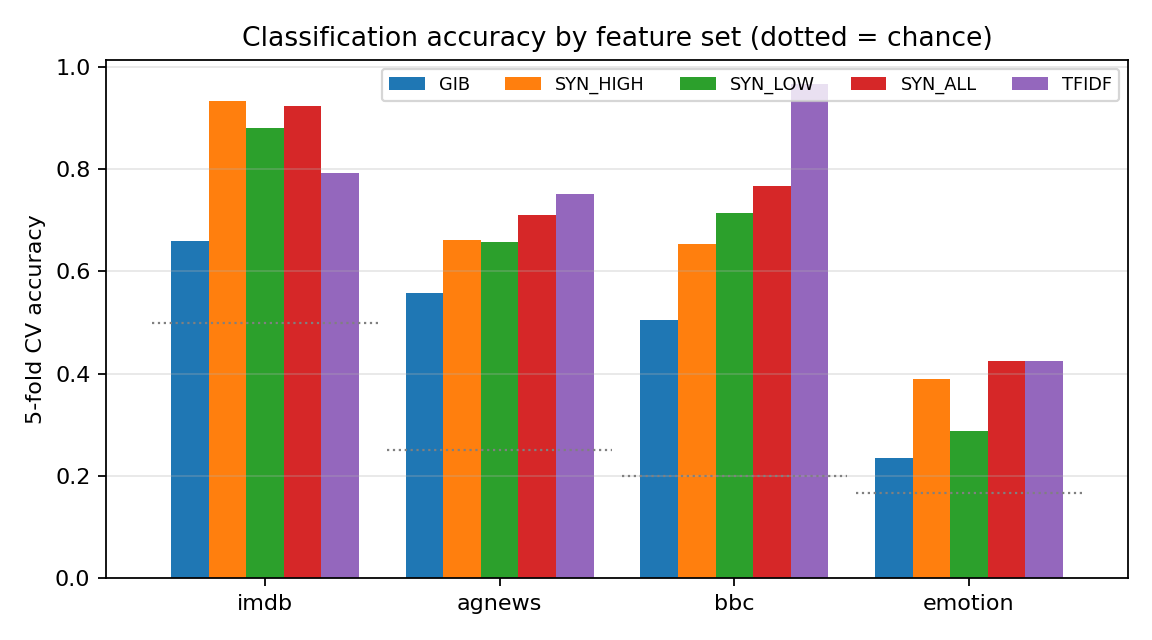
\includegraphics[width=\linewidth]{images/group_accuracy.png}
\caption{Accuracy by feature set. Synesthetic sets (\textsc{low}, \textsc{high}, \textsc{all}) clearly exceed the gibberish control (\textsc{gib}) and chance (dotted) on all four datasets.}
\label{fig:groups}
\end{figure}

\paragraph{Every sense carries information.}
Figure~\ref{fig:sense} breaks the low-polysemy set down by sense ($4$ features each). On every dataset, every sense is informative above chance---including ``smell'' and ``hearing'' for topic classification. Sight is the most informative modality, but no modality is inert. Whatever the model is doing, it is not confined to one privileged sensory axis.

\begin{figure}[t]
\centering
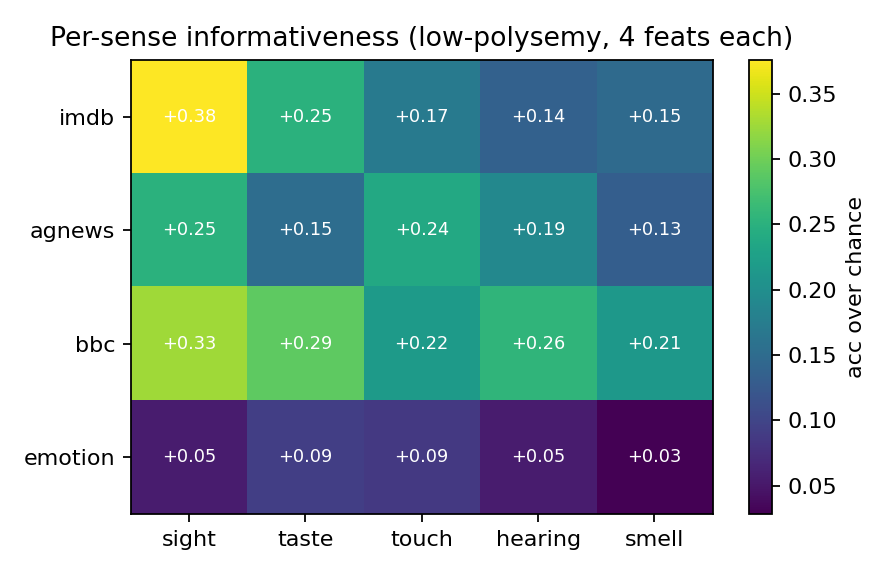
\includegraphics[width=\linewidth]{images/per_sense_heatmap.png}
\caption{Per-sense informativeness of the low-polysemy probes (accuracy over chance, 4 features per sense). All senses help on all tasks.}
\label{fig:sense}
\end{figure}

\paragraph{Usefulness depends only weakly on metaphoricity.}
\label{sec:meta}
Figure~\ref{fig:meta} relates each synesthetic question's univariate usefulness (mean over-chance accuracy across datasets) to its model-rated metaphoricity. There is a positive but moderate correlation (Pearson $r=0.49$, $p<0.01$; $r=0.56$ for our a-priori scores): conventionalized metaphors are individually somewhat stronger features, mostly because affective tasks (IMDB, Emotion) reward predicates like \emph{warm} or \emph{bitter}. But the low-metaphoricity predicates---which carry no figurative meaning and could only be answered by an act of perception the model never performed---remain informative, with most lying above the gibberish baseline and the low-polysemy \emph{set} beating gibberish on every dataset (mean over-chance $0.070$ vs.\ $0.058$ for single probes, and $+0.15$ to $+0.21$ at the set level).

\paragraph{Features are complementary.}
To check that the synesthetic questions are not merely redundant copies of one another, we add the $20$ low-polysemy features in a \emph{random} order and average over $10$ orderings (Figure~\ref{fig:curves}). Accuracy rises steadily all the way to the full set on every dataset, and almost every single-feature addition yields an improvement ($100\%$ of steps on AG~News, $95\%$ on BBC, $89\%$ on IMDB, $79\%$ on Emotion). Each low-polysemy probe thus tends to add information not already captured by the others, rather than re-encoding a single underlying axis.

\paragraph{Comparison with zero-shot.}
Table~\ref{tab:zeroshot} compares the trained synesthetic classifiers with direct \emph{zero-shot} classification, in which the model is shown the task and the candidate labels (a closed-set multiple-choice probe). Zero-shot is the natural upper reference and is strong on sentiment and topic. Yet features built only from sensory questions that \emph{never mention the task} recover most of this accuracy---matching zero-shot to within two points on IMDB ($.92$ vs.\ $.95$)---which suggests the synesthetic probes tap the same information the model uses when classifying directly. Logistic regression and a $64$-unit MLP give nearly identical numbers, confirming that the signal lies in the features, not in classifier capacity.

\begin{table}[t]
\centering\small
\setlength{\tabcolsep}{4.5pt}
\begin{tabular}{lcccccc}
\toprule
 & & zero & \multicolumn{2}{c}{\textsc{low} (20)} & \multicolumn{2}{c}{\textsc{all} (40)} \\
\cmidrule(lr){4-5}\cmidrule(lr){6-7}
 & chance & shot & lr & mlp & lr & mlp \\
\midrule
IMDB     & .50 & .95 & .88 & .87 & .92 & .93 \\
AG News  & .25 & .84 & .66 & .66 & .71 & .70 \\
BBC      & .20 & .92 & .71 & .71 & .77 & .78 \\
Emotion  & .17 & .50 & .29 & .30 & .42 & .37 \\
\bottomrule
\end{tabular}
\caption{Zero-shot direct classification (the model is shown the task) vs.\ classifiers trained on synesthetic features (which never mention the task), with logistic regression (\textsc{lr}) and a $64$-unit MLP. Features recover much of the zero-shot accuracy, and \textsc{lr}$\approx$MLP.}
\label{tab:zeroshot}
\end{table}

\begin{figure}[t]
\centering
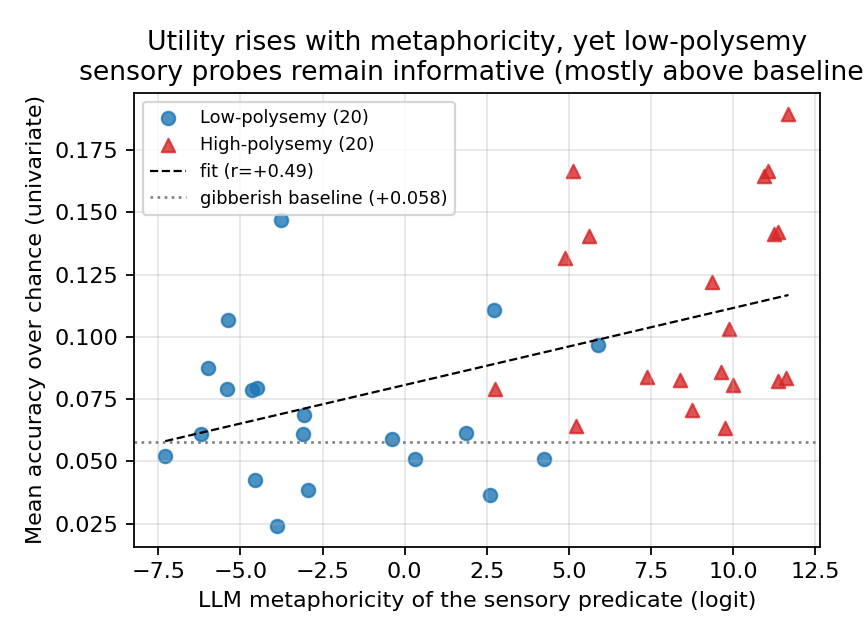
\includegraphics[width=\linewidth]{images/metaphoricity_llm_scatter.png}
\caption{Feature usefulness vs.\ model-rated metaphoricity. The relation is positive but moderate; low-polysemy probes (blue) stay informative even with no figurative meaning.}
\label{fig:meta}
\end{figure}

\begin{figure*}[t]
\centering
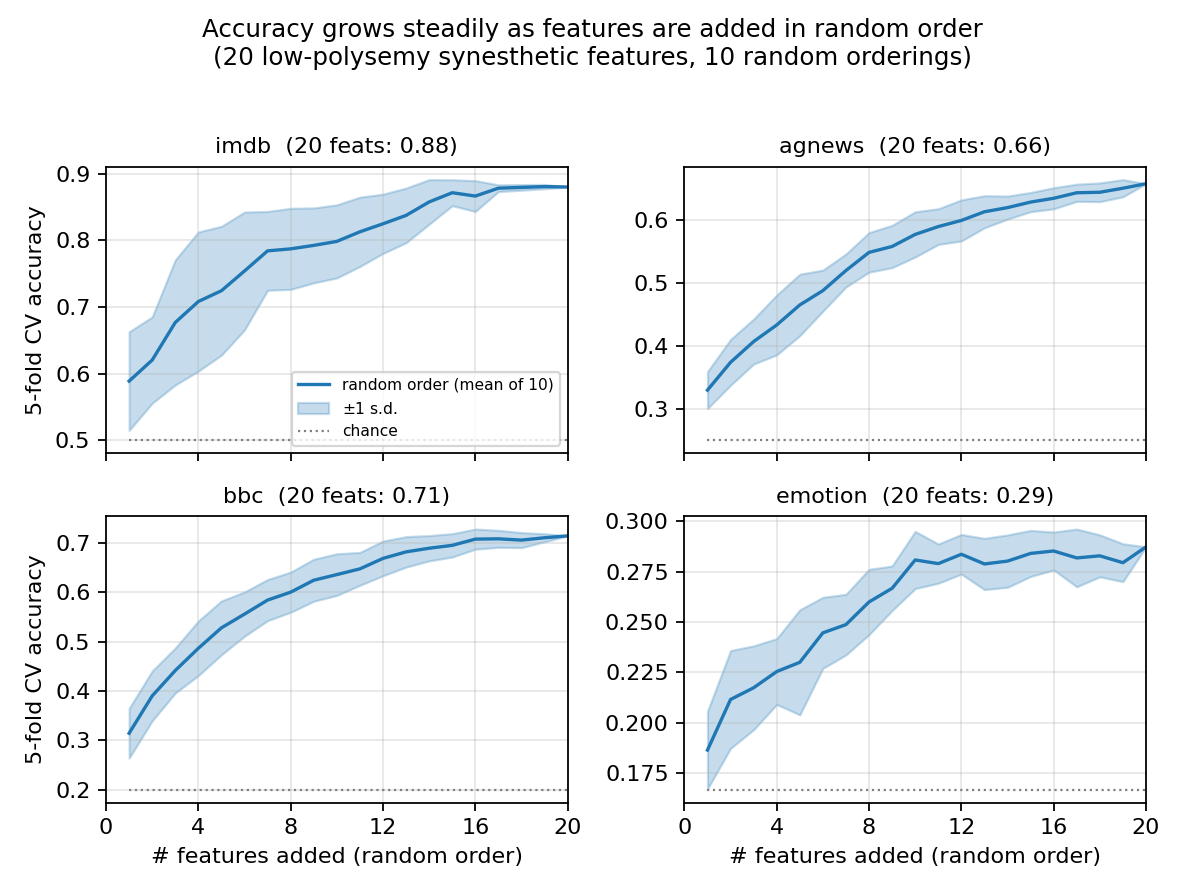
\includegraphics[width=0.92\textwidth]{images/random_order_curves.png}
\caption{Accuracy as the $20$ low-polysemy synesthetic features are added in a \emph{random} order ($10$ random orderings; mean and $\pm1$ s.d.\ band). The steady rise---almost every single-feature addition improves accuracy ($100\%$ of steps on AG~News, $95\%$ on BBC, $89\%$ on IMDB)---indicates that the features are largely complementary: each one tends to contribute information not already captured by the others.}
\label{fig:curves}
\end{figure*}

\section{Discussion: there is no referent}
Why should ``is this text purple?'' carry information about whether a review is positive? Our answer is semiotic rather than perceptual.

For \citet{saussure1916cours}, a sign takes its value from its differential position in the language system, and the referent---the thing in the world---is set aside. A model trained only on text is the limiting case of this picture: it has access to signifiers and their distributional relations \citep{firth1957synopsis}, and to nothing else. It has no referent. Consequently, a sensory predicate is not constrained by any perceptual fact. ``Purple'', ``acidic'' and ``rough'' are not, for the model, attempts to report a perception; they are signifiers that acquire a stable value purely through their differences from other signifiers. Asking the model whether a text is purple is therefore not a category error from its point of view: it is a well-formed question about position in \emph{la langue}, and it receives a graded, text-dependent answer.

This reframes what ``synesthesia'' means here. Synesthesia presupposes \emph{bridges} between modalities; but the model has only one modality (text), so there are no modalities to bridge. What looks like synesthesia is the collapse of every sensory axis onto a single semiotic plane, where ``red'', ``acid'' and ``rough'' are signifiers like any other. The senses place no constraint on the language of the model: a red text is exactly as sayable as an acidic or a smooth one.

Two observations support this reading rather than a ``it is just lexicalized metaphor'' alternative. First, the effect survives when figurative meaning is removed: low-metaphoricity predicates still classify (Figure~\ref{fig:meta}). Second, the information is not generic---gibberish probes, which are also signifiers but lack a richly structured differential value, are markedly weaker (Figure~\ref{fig:groups}). The value of ``purple'' comes neither from a referent (there is none) nor necessarily from a dead metaphor, but from the structured place the word occupies in the system. We do not claim the model escapes language: the consistency of its answers may itself reflect humans' own synesthetic usage in the training corpus---there is, in a sense, no outside-the-text \citep{derrida1967grammatologie}. That is precisely the point.

\section{Conclusion}
Twenty questions about the taste, colour and texture of a text are enough to classify it well above chance and a strong random-word control, with only a weak dependence on whether the sensory words carry figurative meaning. We read this as evidence that, for a referent-free model, sensory predicates are unconstrained signifiers whose usefulness derives from differential structure alone---an empirical illustration of the Saussurean sign without a referent.

\section*{Limitations}
We study one model family and four English datasets with $500$-example subsets; absolute numbers will vary with model and sample size. Our metaphoricity measures (author a-priori and model self-rating) are proxies and could be complemented by human norms such as the Lancaster Sensorimotor Norms \citep{lynott2020lancaster}. The gibberish control equalizes ``probe-ness'' but not lexical frequency or syntactic form. Finally, we cannot fully separate ``no referent'' from ``the training corpus already contains human synesthetic usage''; we take this entanglement to be constitutive of the phenomenon rather than a confound to be removed.

\bibliography{mybib,custom}

\appendix
\section{Question sets}
\label{sec:appendix}
\paragraph{Low-polysemy (per sense).} \emph{Sight:} orange, purple, angular, opaque. \emph{Taste:} salty, umami/savory, starchy, minty. \emph{Touch:} wet, grainy, fuzzy, spongy. \emph{Hearing:} muffled, echoey, nasal, squeaky. \emph{Smell:} metallic, smoky, floral, musty.
\paragraph{High-polysemy (per sense).} \emph{Sight:} dark, bright, colorful, black. \emph{Taste:} sweet, bitter, sour, bland. \emph{Touch:} warm, cold, rough, smooth. \emph{Hearing:} loud, quiet, shrill, harmonious. \emph{Smell:} stinking, fragrant, fishy, fresh.
\paragraph{Form.} Each question is asked as: ``\textit{[text]}\textbackslash n\textbackslash nQuestion: Is this text \textit{[predicate]}?\textbackslash nAnswer with only `yes' or `no'.'' and the feature is $\mathrm{logit(yes)}-\mathrm{logit(no)}$.

\end{document}
